\documentclass[book.tex]{subfiles}
\begin{document}

id Software was funded during February 1991 by four people: 

 \begin{figure}[H]
\centering  
\begin{tabularx}{\textwidth}{ X  X  X  }
  \toprule
  \textbf{Name} &  \textbf{Age} & \textbf{Occupation} \\
  \toprule 
   John Carmack & 22 &  Technical Director\\
   John Romero & 25 &  Level Artist\\
   Adrian Carmack & 22 &  Artist\\
   Tom Hall & 28 &  Game Designer\\
     \toprule
\end{tabularx}
\caption{id Software founding members.}\label{fig:Id Software team}
\end{figure}

Wolfenstein 3D would be the first title for id but the team had already shipped no less than 13 games will working for their previous employer SoftDisk:\\
\begin{itemize}
  \item Dangerous Dave (1988)\footnote{Dangerous Dave is a solo project of John Romero predating Id's formation, but Id Software produced its first sequel and it is sometimes regarded as an early Id Software title. Later Dangerous Dave sequels were not made by Id, nor were later Catacomb titles.}
  \item Commander Keen
  \begin{itemize}
    \item Episode 1: Marooned on Mars (1990)
    \item Episode 2: The Earth Explodes (1991)
    \item Episode 3: Keen Must Die (1991)
    \item Keen Dreams (1991)
    \item Episode 4: Secret of the Oracle (1991)
    \item Episode 5: The Armageddon Machine (1991)
    \item Episode 6: Aliens Ate My Baby Sitter (1991)
  \end{itemize}
  
  \item Dangerous Dave in the Haunted Mansion (1991)
  \item Rescue Rover (1991)
  \item Rescue Rover 2 (1991)
  \item Shadow Knights (1991)
  \item Hovertank 3D (1991)
  \item Catacomb 3D: A New Dimension (1991)
\end{itemize}


Considering the magnitude and ambitions of the title, four more people were added to the team for a total of eight people.\\

 \begin{figure}[H]
\centering  
\begin{tabularx}{\textwidth}{ X  X  X  }
  \toprule
  \textbf{Name} &  \textbf{Age} & \textbf{Occupation} \\
  \toprule 
   Jay Wilbur & ?? &  Business\\
   Kevin Cloud & 27 &  Computer Artist\\
   Robert Prince & ?? &  Composer\\
   Jason Blochowiak & ?? &  Additional Programming\\
     \toprule
\end{tabularx}
\caption{id Software new hires.}\label{fig:Id Software hires}
\end{figure}

Every member was working with an high end 386 DX. As for combining game, tools and assets:\\

 \begin{fancyquotes}
We started with floppy data transfer, but we had a Novell network on coax Ethernet by the end. We didn't have a version control system.  Surprisingly, we went all the way to Quake 3 without one, then we started using Visual Source Safe.\\
 \\
\textbf{John Carmack - Programmer}
\end{fancyquotes}
\section{Programming}

John Carmack took care of most of the runtime code. John Romero programmed many of the tools (editor, packers, …). Jason Blochowiak was contracted to write important subsystems of the game (Input manager, Page Manager, Sound Manager, User Manager).\\
\\
The compiler was Borland C++ 3.1. To compensate for the tiny CRT, some of the developers used two screens (a very unusual thing at the time).\\
\begin{fancyquotes}
At that point, we wanted 21" monitors, but couldn't justify them.  I used a second mono monitor to allow Turbo Debugger 386 to keep the main screen in graphics mode while I stepped through the code.\\
 \\
\textbf{John Carmack - Programmer}
\end{fancyquotes}
\\
Picture of dual head. Monochrome second screen.

Amazingly possible to recreate with DosBox


\begin{fancyquotes}
Jason was part of Id at the start, but we parted ways during Wolf development.
 \bigskip \\
\textbf{John Carmack - Programmer}
 \end{fancyquotes}
 
 
 
\section{Graphics assets}
The graphic assets comprise many aspects of the game:
\begin{itemize}
\item 2D Menus items.
\item 2D Action phase items.
\item Wall textures.
\item entities animations.
\end{itemize}
Those were the work of Adrian Carmack and Kevin Cloud. All of the work was done with Deluxe Paint on highend 386 DX computers. The greatest task was not to draw everything but to make the key decision of what colors would go in the palette.\\
\\
Palette IMAGE\\
\\
\begin{fancyquotes}
We didn't have any scanning tools at the time.\\
\\
\textbf{John Carmack - Programmer}
\end{fancyquotes}
Did they at least had a stylus or something like that ?	\\
\begin{figure}[H]
\centering
 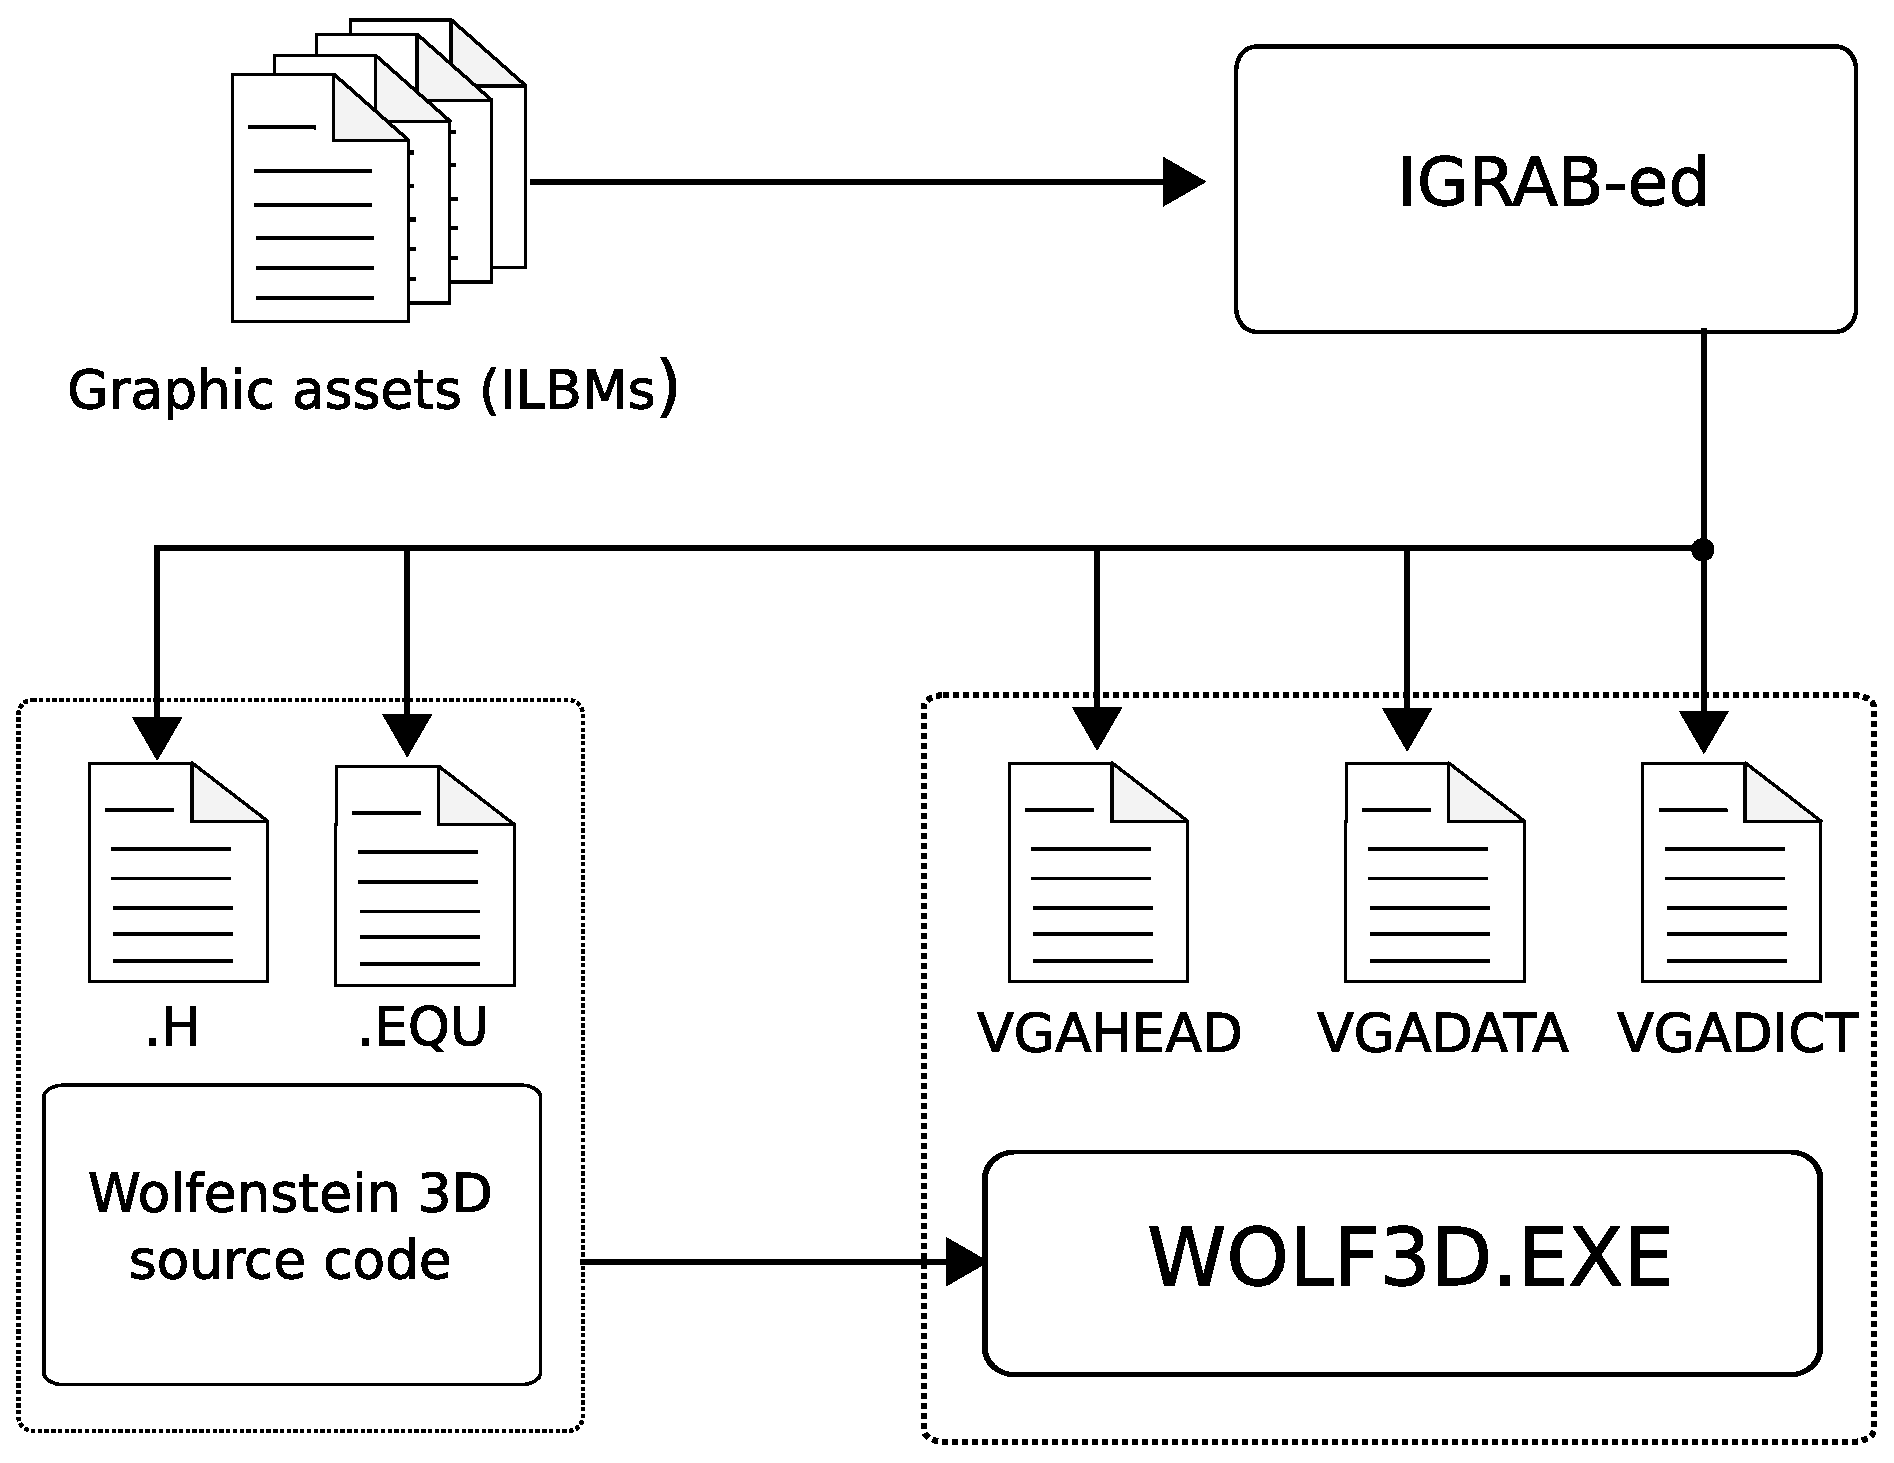
\includegraphics[scale=0.4]{imgs/drawing_plain.eps}
 \caption{Integer layout.} \label{fig:mips}
 \end{figure}

\section{Maps}
Everybody worked a little bit on the map but those were mostly the work of John Romero and Tom Hall. John Romero updated the editor TileEDitor (TED). Maps were plans based, 64x64.
\section{Business}
Jay Wilbur
\section{Sounds}
Robert Prince
\section{Distribution}
Finally after having descrived all the assets created by the team I wanted to discuss a little bit about the distribution model and its intrinsics. Since id Software wanted to distribute the game as a shareware, it was paramount to make the game very easy to copy and exchange among people. So the decision was made to make the game fit on one single disk. This had several consequences:
- Few files
- Compression
- Archives
	\subsection{Compression}
	\subsection{Shareware model}
\end{document}




